\documentclass[conference, a4paper]{IEEEtran}
%\IEEEoverridecommandlockouts
% The preceding line is only needed to identify funding in the first footnote. If that is unneeded, please comment it out.
\usepackage{cite}
\usepackage{amsmath,amssymb,amsfonts}
\usepackage{algorithm}
\usepackage{algorithmic}
\usepackage{graphicx}
\usepackage{textcomp}
\usepackage{xcolor}
\usepackage{systeme}
%\usepackage{IEEEtrantools}
\def\BibTeX{{\rm B\kern-.05em{\sc i\kern-.025em b}\kern-.08em
    T\kern-.1667em\lower.7ex\hbox{E}\kern-.125emX}}

% Custom Additions
\usepackage{datetime}
\usepackage{physics}
\usepackage{mleftright}
\usepackage{optidef}
\usepackage{hyperref}
\usepackage{cleveref}
\usepackage{xfrac}
\usepackage{caption,subcaption}
%\usepackage[utf8]{inputenc}
%\usepackage[english]{babel}
%\usepackage{float}

\newtheorem{theorem}{Theorem}[section]

\begin{document}

\title{A Consumer Appliance-Level Framework\\for Optimized Load Shedding}

\author{
	\IEEEauthorblockN{
		Christian Y. Cahig\IEEEauthorrefmark{1}, Abdul Aziz G. Mabaning\IEEEauthorrefmark{2}
	}
	\IEEEauthorblockA{
		\textit{Department of Electrical Engineering and Technology, College of Engineering and Technology}\\
		\textit{Mindanao State University - Iligan Institute of Technology}\\
		Iligan City, Philippines\\
		\IEEEauthorrefmark{1}chriscahig@gmail.com,
		\IEEEauthorrefmark{2}mraaguevarra@gmail.com
	}
}

\maketitle

%\noindent
%\textit{Updated as of {\today\ \currenttime}.}\\

\begin{abstract}
Lorem ipsum
\end{abstract}

\begin{IEEEkeywords}
Optimization, power systems, optimal load shedding.
\end{IEEEkeywords}


\section{Introduction}
\label{sec: Introduction}

Load shedding is a course of action a utility company can take
when the balance between power supply and demand is at risk \cite{Jabian2018},
or when the system voltage or frequency exceeds its allowable lower limit for more than a minute \cite{GMC2016}.
Compared to investing on the installation of generating capacities to curb threats on the supply-demand balance,
load shedding is more economical and realistic in short-term considerations.

Since this strategy directly deals with the customers, load shedding has to be an optimized process.
As such, one can find numerous works in literature
(\textit{e.g.},
fast load shedding \cite{Wester2014},
clustering-based load shedding \cite{Potel2019}, and
load shedding during disaster events \cite{Babaei2020})
on feeder-level implementations.
In this setting, the smallest ``sheddable" unit of load is the total load connected to a feeder.
This coarse treatment is prone to excessive shedding of load and an unoptimized utilization of available supply.
Accordingly, we see works on residence-level implementation:
\textit{e.g.},
using smart meters, single-board computers, server monitoring \cite{Bhattacherjee2019},
detecting rate-of-change of frequency \cite{Sigrist2015},
and using a mobile distribution-level PMU \cite{Yao2020}.

Moving forward in this trend, \cite{Jabian2020} proposed a shedding framework where the smallest ``sheddable" unit of load is a consumer appliance.
This granular scheme addresses the concern of excessive load dropping in a feeder-level implementation,
as well as improves the operation of a residence-level setup.
Keeping both the utility and the customer in the framework means both parties can make the most of the situation in their perspectives.
By having the ability to prioritize appliances according to personal judgment, a consumer can avoid total interruption of comfort and/or productivity within his/her premises.
On the other hand, the utility can maximize the utilization of available power supply.

This work 

The remainder of the paper proceeds as follows.
\textit{\textbf{Lorem ipsum}}

\section{Basic Problem Formulation}
\label{sec: Basic Problem Formulation}

This section \textit{\textbf{blahblah}}

\subsection{System Configuration}
\label{subsec: II--System Configuration}

Consider a distribution system with $C$ loads (see Fig. \ref{figIV-01}),
where each load $c$ represents a consumer (\textit{i.e.}, a registered customer of the utility).
We assume a communication network that is not wholly centralized:
(i) appliances within the premises of consumer $c$ are monitored and controlled by consumer node $\mathsf{K}_{c}$;
(ii) all consumer nodes communicate with central node $\mathsf{U}$ in the utility side (\textit{e.g.}, housed in a substation); and
(iii) communication between $\mathsf{K}_{c}$'s and $\mathsf{U}$ have a bidirectional protocol.

\begin{figure}[t!]
	\centering
	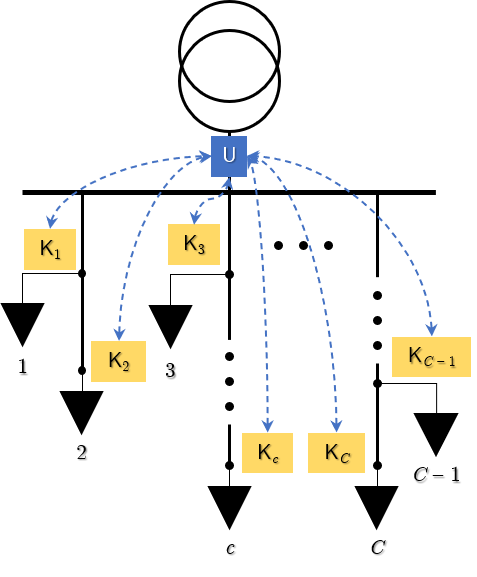
\includegraphics[scale=0.75]{figure-IV-01.png}
	\caption{System single line diagram and network topology for the consumer appliance-level load shedding.
	Although the figure depicts one load at each node for brevity, the framework presented is not limited to three-phase loads.}
	\label{figIV-01}
\end{figure}

For the appliance-level shedding to be possible, a consumer $c$ assigns $P_{c}$ priority levels, according to his/her preference and prerogative (see Fig. \ref{figIV-02}).
In this case, we take $p=1$ as the highest priority of being supplied---\textit{i.e.},
appliances within this priority level are to be supplied first when possible---and
$p=P_{c}$ as the least priority.
There are $M_{p}$ appliances within level $p$, and each of them are denoted by $d_{c,i}^{\left(p\right)}$.
Without introducing another variable, let us use $d_{c,i}^{\left(p\right)}$ as the power rating of that appliance.
We can then represent the appliances in level $p$ by a vector of its power ratings $\mathbf{d}_{c}^{\left(p\right)} \in \mathbb{R}^{M_{p}}$
and the appliances within consumer $c$ as a vector $\mathbf{d}_{c} \in \mathbb{R}^{M_{1} + \ldots + M_{P_{c}}}$,
that is,
\begin{IEEEeqnarray}{rCl}
	\mathbf{d}_{c}^{\left(p\right)} &=& \left[ d_{c,1}^{\left(p\right)}, d_{c,2}^{\left(p\right)}, \ldots, d_{c,M_{p}}^{\left(p\right)} \right]^{\intercal} \\
	\label{eqn27}
	\mathbf{d}_{c} &=& \left[ \mathbf{d}_{c}^{\left(1\right)}, \mathbf{d}_{c}^{\left(2\right)}, \ldots, \mathbf{d}_{c}^{\left(P_{c}\right)} \right]^{\intercal}
	\label{eqn28}
\end{IEEEeqnarray}
It follows that consumer $c$ has $\sum_{i=1}^{P_{c}} M_{i}$ appliances
whose active power ratings add up to
\begin{equation*}
	\sum_{p=1}^{P_{c}} \sum_{i=1}^{M_{p}} d_{c,i}^{\left(p\right)}
\end{equation*}

\begin{figure}[t!]
	\centering
	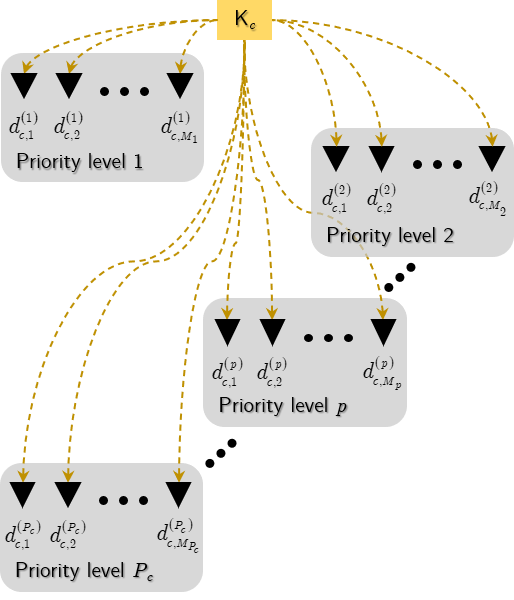
\includegraphics[scale=0.75]{figure-IV-02.png}
	\caption{Grouping of appliances into priority levels for consumer $c$.}
	\label{figIV-02}
\end{figure}

\subsection{Nominating Appliances for Load Shedding}
\label{subsec: II--Nominating Appliances for Load Shedding}

In the event where load shedding has to be implemented, the utility has to determine how much load needs to be shed.
If the expected available supply for the system during the impending shedding period is $S_{\text{sys}}$,
and the expected total load during the same period is $L_{\text{sys}}$,
then we can define a \textit{reduction ratio} $\rho$ as
\begin{equation}
	\rho = \frac{S_{\text{sys}}}{L_{\text{sys}}}
	\label{eqn29}
\end{equation}
Assuming a load shedding scenario where $S_{\text{sys}}$ may not meet $L_{\text{sys}}$,
$\rho$ is the fraction of $L_{\text{sys}}$ that must be shed.
This means that a consumer has to adjust his/her consumption by $\rho - \mu$,
where $\mu$ is a correcting margin\footnote{
$\mu$ can be set as the maximum forecasting error that is likely to happen,
\textit{e.g.}, 95\% of errors in the system's forecast records do not exceed this value.}
determined by the utility to compensate for load forecast errors.
Both $\rho$ and $\mu$ are then communicated by $\mathsf{U}$ to all $\mathsf{K}_{c}$'s.

\begin{figure}[t!]
	\centering
	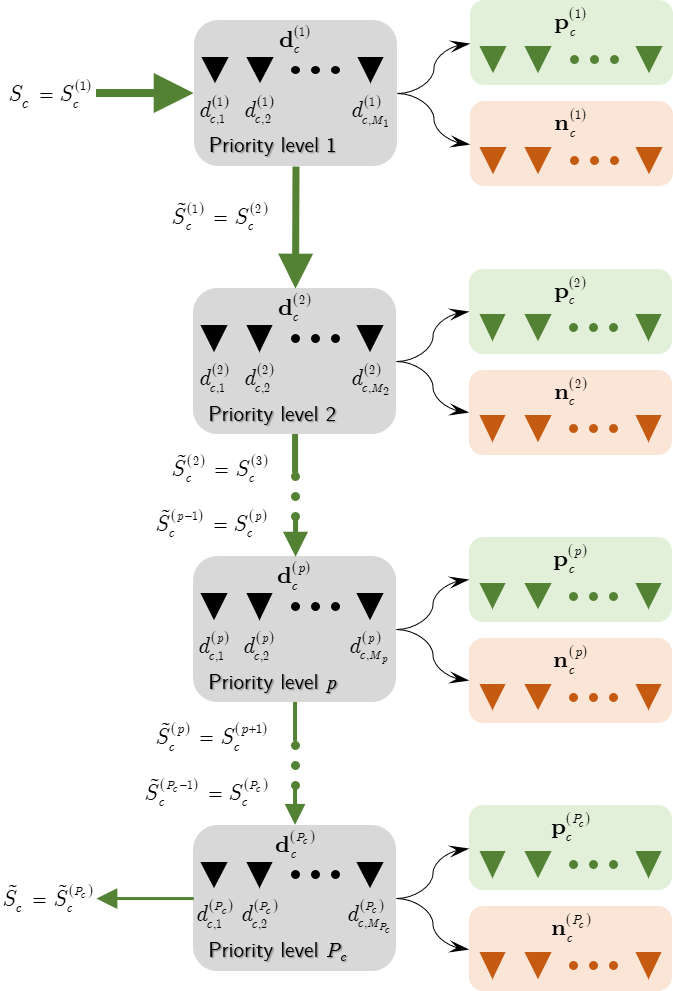
\includegraphics[scale=0.75]{figure-IV-03.png}
	\caption{Utilization of $S_{c}$ among the appliances of consumer $c$.}
	\label{figIV-03}
\end{figure}

For a consumer $c$, whose total consumption at the moment $\mathsf{K}_{c}$ receives $\rho$ and $\mu$, is $L_{c}$,
his/her expected supply for the shedding period, $S_{c}$, is given by
\begin{equation}
	S_{c} = \left( \rho - \mu \right) L_{c}
	\label{eqn30}
\end{equation}
$\mathsf{K}_{c}$ has to maximize the utilization of $S_{c}$ among all appliances it oversees
according to the priority levels (see Fig. \ref{figIV-03}).
At $p=1$, the supply $S_{c}^{\left(1\right)} = S_{c}$ is optimally distributed among appliances $\mathbf{d}_{c}^{\left(1\right)}$.
This results in two groups of appliances for $p=1$:
those that are to be supplied ($\mathbf{p}_{c}^{\left(1\right)}$),
and those that are nominated for shedding ($\mathbf{n}_{c}^{\left(1\right)}$).
Because appliance ratings are fixed and considered indivisible, we can retrieve $\tilde{S}_{c}^{\left(1\right)}$,
which is the portion of $S_{c}^{\left(1\right)}$ that is not allocated to power any more appliances at $p=1$.
Then, $\tilde{S}_{c}^{\left(1\right)}$ becomes the supply to be optimally distributed among appliances at $p=2$
(\textit{i.e.},
$S_{c}^{\left(2\right)} = \tilde{S}_{c}^{\left(1\right)}$)
and the process continues through $p=P_{c}$.
The unallocated supply at the lowest priority level is also the unallocated portion of $S_{c}$,
\textit{i.e.}, $\tilde{S}_{c} = \tilde{S}_{c}^{\left(P_{c}\right)}$.
We can define a vector for all appliances in $c$ nominated for shedding:
\begin{equation}
	\mathbf{n}_{c} = \left[ \mathbf{n}_{c}^{\left(1\right)}, \mathbf{n}_{c}^{\left(2\right)}, \ldots, \mathbf{n}_{c}^{\left(P_{c}\right)} \right]^{\intercal}
	\label{eqn31}
\end{equation}
Then, $\mathsf{K}_{c}$ reports $\tilde{S}_{c}$ and $\mathbf{n}_{c}$ to $\mathsf{U}$.

\begin{figure}[t!]
	\centering
	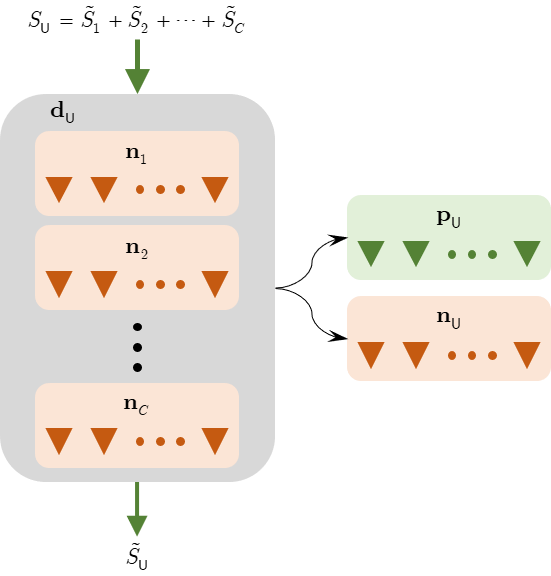
\includegraphics[scale=0.75]{figure-IV-04.png}
	\caption{Utilization of $S_{\mathsf{U}}$ among appliances previously nominated by $\mathsf{K}_{c}$'s.}
	\label{figIV-04}
\end{figure}

Having $\tilde{S}_{c}$ and $\mathbf{n}_{c}$, $\forall c=1,2,\ldots,C$,
%we define the total unallocated supply among all consumers as
we define the total unallocated supply and the vector of appliances nominated for shedding from all consumers as
\begin{IEEEeqnarray}{rCl}
	S_{\mathsf{U}} &=& \sum_{c=1}^{C} \tilde{S}_{c} \\
	\label{eqn32}
	\mathbf{d}_{\mathsf{U}} &=& \left[ \mathbf{n}_{1}, \mathbf{n}_{2}, \ldots, \mathbf{n}_{C} \right]^{\intercal}
	\label{eqn33}
\end{IEEEeqnarray}
To further maximize utilization, $\mathsf{U}$ redistributes $S_{\mathsf{U}}$ among $\mathbf{d}_{\mathsf{U}}$ (see Fig. \ref{figIV-04}).
As with the procedure for each consumer priority level, this results in two groups of appliances:
$\mathbf{p}_{\mathsf{U}}$ contains those in $\mathbf{d}_{\mathsf{U}}$ that are to be supplied using $S_{\mathsf{U}}$,
while $\mathbf{n}_{\mathsf{U}}$ is the final roster of appliances nominated for shedding.
The utility relays $\mathbf{p}_{\mathsf{U}}$ (and/or $\mathbf{n}_{\mathsf{U}}$) to all $\mathsf{K}_{c}$'s;
after which the load shedding implementation commences.

\subsection{Consumer-side Optimization}
\label{subsec: II--Consumer-side Optimization}

At priority level $p$, $\mathsf{K}_{c}$ has to allocate $S_{c}^{\left(p\right)}$ among appliances denoted by $\mathbf{d}_{c}^{\left(p\right)}$.
Each appliance is a quantized load of fixed amount;
hence, $\mathsf{K}_{c}$ can only alter the distribution of $S_{c}^{\left(p\right)}$
by either ``picking up" or nominating for shedding an appliance.
We denote a binary decision variable $k_{i}$
for appliance $d_{c,i}^{\left(p\right)} \in \mathbf{d}_{c}^{\left(p\right)}$
such that
\begin{equation}
	k_{i} =
	\begin{cases*}
		0, & if $d_{c,i}^{\left(p\right)}$ is nominated for shedding \\
		1, & otherwise
	\end{cases*}
	\label{eqn34}
\end{equation}

The amount from $S_{c}^{\left(p\right)}$ that is utilized for ``picking up" appliances is given by
\begin{IEEEeqnarray*}{rCl}
	\sum_{i=1}^{M_{p}} k_{i} d_{c,i}^{\left(p\right)} = k_{1} d_{c,1}^{\left(p\right)} + k_{2} d_{c,2}^{\left(p\right)} + \ldots + k_{M_{p}} d_{c,M_{p}}^{\left(p\right)} = \left(\mathbf{d}_{c}^{\left(p\right)}\right)^{\intercal} \mathbf{k}
\end{IEEEeqnarray*}
where $\mathbf{k} = \left[ k_{1}, k_{2}, \ldots, k_{M_{p}} \right]^{\intercal}$ is the vector representation of the decision variables.
The unallocated portion of $S_{c}^{\left(p\right)}$ is
\begin{IEEEeqnarray}{rCl}
	 \tilde{S}_{c}^{\left(p\right)} = S_{c}^{\left(p\right)} - \sum_{i=1}^{M_{p}} k_{i} d_{c,i}^{\left(p\right)} = S_{c}^{\left(p\right)} - \left(\mathbf{d}_{c}^{\left(p\right)}\right)^{\intercal} \mathbf{k}
	 \label{eqn35}
\end{IEEEeqnarray}
Hence, optimizing the utilization of $S_{c}^{\left(p\right)}$ corresponds to minimizing $\tilde{S}_{c}^{\left(p\right)}$.
In this sense, $S_{c}^{\left(p\right)}$ is a ``cost" to be minimized.
Moreover, one has to restrict the picking up of appliances so that $\tilde{S}_{c}^{\left(p\right)}$ is nonnegative, \textit{i.e.},
\begin{equation}
	S_{c}^{\left(p\right)} - \left(\mathbf{d}_{c}^{\left(p\right)}\right)^{\intercal} \mathbf{k} \geq 0
	\label{eqn36}
\end{equation}

From \eqref{eqn34}-\eqref{eqn36}, the consumer-side optimization problem is
\begin{mini!}|l|
	{\mathbf{k}}
	{ \left\{ \tilde{S}_{c}^{\left(p\right)} = S_{c}^{\left(p\right)} - \left(\mathbf{d}_{c}^{\left(p\right)}\right)^{\intercal} \mathbf{k} \right\} }
	{\label{eqn37}}
	{}{}
	\addConstraint{ S_{c}^{\left(p\right)} - \left(\mathbf{d}_{c}^{\left(p\right)}\right)^{\intercal} \mathbf{k} \geq 0 }
	\addConstraint{ k_{i} \in \left\{0,1\right\},\ i=1,2,\ldots,M_{p}  }
\end{mini!}
The solution to \eqref{eqn37}, $\mathbf{k}^{\ast}$, is the switching combinations for appliances $\mathbf{d}_{c}^{\left(p\right)}$ that minimizes $\tilde{S_{c}}^{\left(p\right)}$.
Moreover, \eqref{eqn37} is performed at each priority level $p$ of each consumer $c$.

\subsection{Utility-side Optimization}
\label{subsec: II--Utility-side Optimization}

In simplistic terms, utility-side optimization seeks to ``squeeze" out more utilization of supply.
The intuition is that $\tilde{S_{c}}$ may be enough to pick up some appliances in $\mathbf{n}_{b}$, $b \neq c$.
The distribution of $S_{\mathsf{U}}$ among $\mathbf{d}_{\mathsf{U}}$ is similar to \eqref{eqn37}.
Each appliance $d_{\mathsf{U},i} \in \mathbf{d}_{\mathsf{U}}$ can only be controlled by $\mathsf{U}$ in two ways.
We define a binary variable $u_{i}$ to indicate this decision parameter:
\begin{equation}
	u_{i} =
	\begin{cases*}
		0, & if $d_{\mathsf{U},i}$ is nominated for shedding \\
		1, & otherwise
	\end{cases*}
	\label{eqn38}
\end{equation}
If $\mathbf{d}_{\mathsf{U}}$ has $M_{\mathsf{U}}$ appliances, then the amount from $S_{\mathsf{U}}$ expended for picking up appliances is given by
\begin{equation*}
	\sum_{i=1}^{M_{\mathsf{U}}} u_{i} d_{\mathsf{U},i} = u_{1} d_{\mathsf{U},1} + u_{2} d_{\mathsf{U},2} + \ldots + u_{M_{\mathsf{U}}} d_{\mathsf{U},M_{\mathsf{U}}} = \left( \mathbf{d}_{\mathsf{U}} \right)^{\intercal} \mathbf{u}
\end{equation*}
where $\mathbf{u}$ is the vector representation of the decision variables,
and $\mathbf{u}, \mathbf{d}_{\mathsf{U}} \in \mathbb{R}^{M_{\mathsf{U}}}$.
The unallocated portion of $S_{\mathsf{U}}$ is
\begin{equation}
	\tilde{S}_{\mathsf{U}} = S_{\mathsf{U}} - \sum_{i=1}^{M_{\mathsf{U}}} u_{i} d_{\mathsf{U},i} = S_{\mathsf{U}} - \left( \mathbf{d}_{\mathsf{U}} \right)^{\intercal} \mathbf{u}
	\label{eqn39}
\end{equation}
where $\tilde{S}_{\mathsf{U}}$ is to be minimized but cannot be negative:
\begin{equation}
	S_{\mathsf{U}} - \left( \mathbf{d}_{\mathsf{U}} \right)^{\intercal} \mathbf{u} \geq 0
	\label{eqn40}
\end{equation}
Finally, the utility-side optimization problem is
\begin{mini!}|l|
	{\mathbf{k}}
	{ \left\{ \tilde{S}_{\mathsf{U}} = S_{\mathsf{U}} - \left( \mathbf{d}_{\mathsf{U}} \right)^{\intercal} \mathbf{u} \right\} }
	{\label{eqn41}}
	{}{}
	\addConstraint{ S_{\mathsf{U}} - \left( \mathbf{d}_{\mathsf{U}} \right)^{\intercal} \mathbf{u} \geq 0 }
	\addConstraint{ u_{i} \in \left\{0,1\right\},\ i=1,2,\ldots,M_{\mathsf{U}}  }
\end{mini!}
The solution to \eqref{eqn41}, $\mathbf{u}^{\ast}$, is the switching combinations for appliances $\mathbf{d}_{\mathsf{U}}$ that minimizes the $\tilde{S}_{\mathsf{U}}$.

\section{A Critique on the Original Work}
\label{sec: A Critique on the Original Work}

While the intent of the work by \cite{Jabian2020} is commendable in adding a demand-response dimension to load shedding,
there are certain points in their methodology that we find insufficiently justified (at least in the paper alone).

First, the prioritized utilization of $S_c$ (see Fig. \ref{figIV-03}) can be recast as a non-cascaded procedure.
For example, the priority levels of appliances
$\mathbf{d}_{c} = \left[ d_{c,1}, d_{c,2}, \ldots, d_{c,N_{c}} \right]^{\intercal}$
can be encoded as a vector of corresponding priority weights
$\mathbf{\Phi}_{c} = \left[ \phi_{c,1}, \phi_{c,2}, \ldots, \phi_{c,N_{c}} \right]^{\intercal}$
where $N_{c} = \sum_{i=1}^{P_{c}} M_{i}$ is the number of appliances in $c$.
In this manner, two appliances $d_{c,i}$ and $d_{c,j}$ are
of the same priority levels if $\phi_{c,i} = \phi_{c,j}$.
Moreover, the consumer-side optimization \eqref{eqn37} need not be performed $P_{c}$ times,
and can be recast as a single-stage minimization of $\tilde{S_{c}}$:
\begin{maxi!}|l|
	{\mathbf{k}}
	{ \left\{ \tilde{S}_{c} = S_{c} - \left( \mathbf{\Phi}_{c} \odot \mathbf{d}_{c} \right)^{\intercal} \mathbf{k} \right\} }
	{\label{eqn-IV-C: Single-stage consumer-side optimization}}
	{}{}
	\addConstraint{ S_{c} - \left( \mathbf{\Phi}_{c} \odot \mathbf{d}_{c} \right)^{\intercal} \mathbf{k} \geq 0 }
	\addConstraint{ k_{i} \in \left\{0,1\right\},\ i=1,2,\ldots,N_{c}  }
\end{maxi!}
where $\odot$ denotes element-wise multiplication,
and $\mathbf{k} = \left[k_{1}, k_{2}, \ldots, k_{N_{c}} \right]$ is a modified vector representation of the decision variables corresponding to $\mathbf{d}_{c}$.
Although there is a burden in properly setting $\mathbf{\Phi}_{c}$,
it is reasonable to wonder whether the computational burden of per-priority level optimization \eqref{eqn37}
is significantly less than that of \eqref{eqn-IV-C: Single-stage consumer-side optimization} or any variants thereof.

Second, the ``rush to heuristics" may have been unjustified at worst and improvable at best.
In \cite{Jabian2020}, genetic algorithm (GA) and binary particle swarm optimization (BPSO)
with modified initialization schemes were used as the solution method.
The consumer-side optimization \eqref{eqn37} is an integer linear programming problem,
which can be solved efficiently by properly chosen numerical approaches.
This makes the authors' claim of GA being more suitable than BPSO for real-time applications
of less confidence;
a better approach would be a comparison of GA and BPSO with performant numerical methods.
Also, the procedure for tuning GA and BPSO parameters
(\textit{e.g.}, population size, mutation rate, crossover rate, inertia weight)
was not discussed.
These parameters are known to affect search performance, hence,
it is reasonable to expect at least an ablation study highlighting the effects of their values.

Lastly, given the implications of future real-life implementation,
the case studies should have included more scenarios
in addition to having ``low" and ``high" diversity of appliance ratings.
Equally pressing scenarios could be varying number of consumers and fixed/varied number of priority levels.
A more serious lapse is that the case studies did not indicate the ground truth optimum values.
This raises a valid concern mainly because GA and BPSO
(among other evolutionary and population-based heuristics)
are known to provide sub-optimal and/or inconsistent results due to reliance on some form of random distribution.

\section{Conclusion}
\label{V. Conclusion}

In this paper, we examined the fundamental theory of what makes a feasible point optimal for a given optimization problem.
Specifically, we discussed the necessary and sufficient conditions for optimality by developing it
from more foundational notions in elementary calculus and linear algebra.
These conditions set a basic pattern for solution methods:
find a stationary point, and verify if it is a local minimizer (\textit{e.g.}, via its Hessian).
We also showed how convex problems are special in the sense that a local minimizer is a global minimizer;
this is the primary reason for advanced strategies that reformulates the problem into a convex form.
Lastly, we presented a modified update to the capstone project on optimal load shedding,
as well as a critique on the original work from which it was derived.

%%%%%%%%%%%%%%%%%%%%%

%\vspace{40pt}
%\section*{Acknowledgment}
%Majority of the material in this paper were referred from the first two chapters of the book \cite{dugan1996electrical}.

%\vspace{40pt}
%\section*{References}
\bibliographystyle{IEEEtran}
%The argument is your BibTeX string definitions and bibliography database(s).
\bibliography{capstone_project}

\end{document}
